% ---------------------------------------------------------------------------------------------------------
% 結果 II：計画は実行できるか（実験 2，3）
% ---------------------------------------------------------------------------------------------------------
\section{結果 II：計画は実行できるか}
\label{sec:exec}
学習した制御器を比べる前に，オラクルの解そのものが環境で実行できるかを調べる．
計画どおりのトルクを加える再生（表~\ref{tab:methods} の REPLAY）で失敗するなら，その原因は学習ではなく計画か実行系にある．

\subsection{再生の分解}
\label{sec:replay}
図~\ref{fig:replay3d} は，$T=18$\,s，$m=66$\,kg，$\phi_\ell=0.25$ の参照解を環境で再生した例である．
この試行は離手，捕捉，2\,s の保持に成功したが，把持利用率の最大値は計画の \refUpeak に対して 1.51 に達した．
計画は実行できるが，計画どおりの負荷では実行できない．
\begin{figure*}[t]
\centering
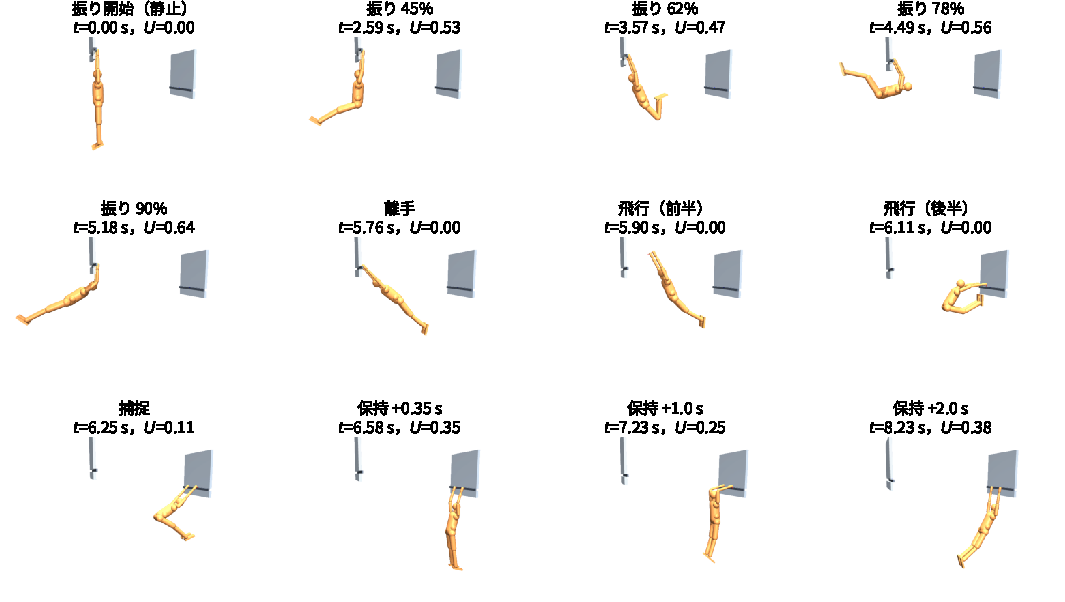
\includegraphics[width=\linewidth]{../results/figs/replay3d.pdf}
\caption{環境での実行例（$T=18$\,s，$m=66$\,kg，$\phi_\ell=0.25$ の参照解の再生；制御周期 2\,ms，共通の着地反射）．
$t$ は振り開始からの時間，$U$ はその瞬間の把持利用率．2\,s の保持まで成功した試行で，最大の把持利用率は 1.51 であった．}
\label{fig:replay3d}
\end{figure*}

再生が失敗する原因を，3 体格（$m=60,66,75$\,kg）の参照解について，軸を一つずつ変えて調べた（図~\ref{fig:replay}，表~\ref{tab:replay}）．
成功は $\Fmax=2600$\,N で 2\,s 保持できた本数で数える．

\textbf{制御周期．}剛体衝突モデルの参照解は，制御周期 1\,ms と 2\,ms では 3 本中 \repImpTwo 本が成功し，5\,ms では \repImpFive 本，
10\,ms では \repImpTen 本（捕捉に至らない）であった．20\,ms では振りの途中で A から滑り落ち，1 本も離手に至らない．
指令を制御周期の間一定に保つことによる時間遅れが，軽い前腕と下腿の速い運動を乱し，手先の力が錐を出るためである．

\textbf{離手時刻．}離手を制御周期の格子に丸めると，2\,ms の周期でも成功は \repImpTwo 本から \repImpRoundTwo 本に減り，
順応捕捉モデルの参照解では \repCompTwo 本から \repCompRoundTwo 本になる．
離手時刻は 1\,ms の精度で合わせる必要がある．以降の実験では離手を計画の時刻に正確に合わせる．

\textbf{積分刻み．}積分刻みを 1，0.5，0.25\,ms と変えても，離手・捕捉・保持の成否はほとんど変わらない．
ただし捕捉直後の把持利用率の最大値は刻みによって最大 \subdtUspread\,\%変わり，1\,\%の精度では収束していない．
捕捉の衝撃は，この環境の接触モデルでは積分刻みに敏感である．

\textbf{計画のメッシュ．}計画の離散化を半分の粗さにすると，どちらの捕捉モデルでも成功は 0 本になる．
2 倍に細かくすると，振りの関節角の追従誤差の中央値は \meshErrOne $\times10^{-2}$\,rad から \meshErrTwo $\times10^{-2}$\,rad に半減し，
順応捕捉モデルの参照解は 3 本すべてが 2\,s の保持に至った（標準のメッシュでは \repCompMeshOneHeld 本）．
ただし把持利用率が 2 を超える試行があり，$\Fmax=2600$\,N での成功は \repCompMeshTwo 本である．
最適化が返す解は離散化した問題の解であり，連続時間の力学の解ではない．その差が再生の失敗の主な原因の一つである．
半分の粗さのメッシュで解いた $\Upk$ は 2 倍に細かいメッシュの値と最大 \meshUhalf\,\%違う．

\textbf{開始相．}順応捕捉モデルの参照解は，捕捉の瞬間から始めれば 3 本すべてが成功するが，
飛行の開始から始めると \repCompStartFlight 本，静止から始めると \repCompTwo 本である．
失敗は振りの誤差が飛行を通じて捕捉の幾何に伝わることで起きている．
\begin{figure*}[t]
\centering
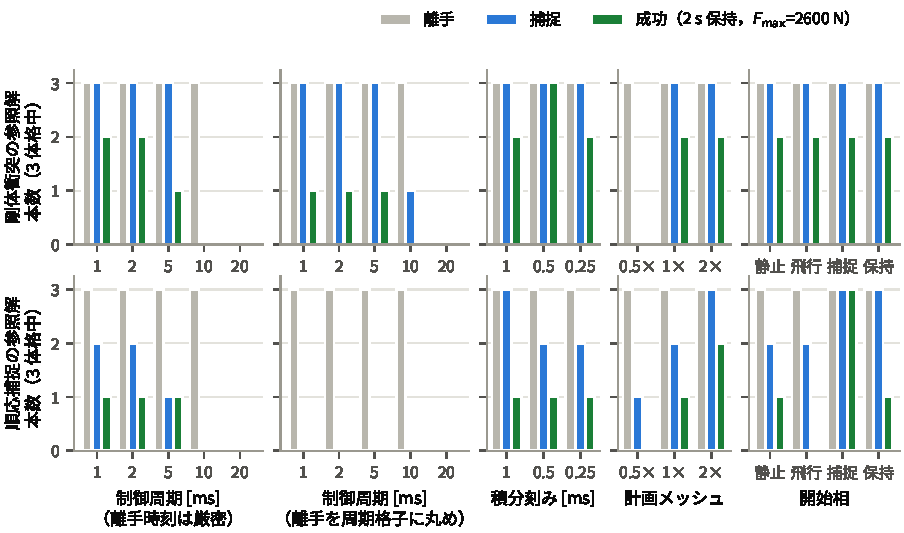
\includegraphics[width=\linewidth]{../results/figs/x2_replay.pdf}
\caption{再生の分解（実験 2）．上段は剛体衝突モデル，下段は順応捕捉モデルの参照解で，縦軸は 3 体格のうち各段階に至った本数．
左から，制御周期（離手は計画の時刻に正確に合わせる），制御周期（離手を周期の格子に丸める），積分刻み，計画のメッシュ，開始相．
特に断らない軸は，制御周期 2\,ms，積分刻み 0.25\,ms，標準のメッシュ，静止からの開始である．}
\label{fig:replay}
\end{figure*}
\begin{table*}[t]
\centering\scriptsize
\caption{再生の分解の全結果（図~\ref{fig:replay} の数値）．$n$ は参照解の本数．成功は $\Fmax=2600$\,N で 2\,s 保持できた本数．}
\label{tab:replay}
\IfFileExists{tab_x2.tex}{\resizebox{0.86\textwidth}{!}{\begin{tabular}{lllrrrrrr}
\toprule
参照解 & 分解の軸 & 設定 & $n$ & 離手 & 捕捉 & 2 s 保持 & 成功 & 振り追従誤差 [$10^{-2}$ rad] \\
\midrule
剛体衝突 & 制御周期 [ms] & 1 & 3 & 3 & 3 & 3 & 2 & 3.9 \\
剛体衝突 & 制御周期 [ms] & 2 & 3 & 3 & 3 & 3 & 2 & 3.8 \\
剛体衝突 & 制御周期 [ms] & 5 & 3 & 3 & 3 & 1 & 1 & 3.5 \\
剛体衝突 & 制御周期 [ms] & 10 & 3 & 3 & 0 & 0 & 0 & 3.0 \\
剛体衝突 & 制御周期 [ms] & 20 & 3 & 0 & 0 & 0 & 0 & 13.7 \\
剛体衝突 & 制御周期 [ms]（丸め） & 1 & 3 & 3 & 3 & 2 & 1 & 3.9 \\
剛体衝突 & 制御周期 [ms]（丸め） & 2 & 3 & 3 & 3 & 2 & 1 & 3.8 \\
剛体衝突 & 制御周期 [ms]（丸め） & 5 & 3 & 3 & 3 & 1 & 1 & 3.7 \\
剛体衝突 & 制御周期 [ms]（丸め） & 10 & 3 & 3 & 1 & 0 & 0 & 4.1 \\
剛体衝突 & 制御周期 [ms]（丸め） & 20 & 3 & 0 & 0 & 0 & 0 & 13.7 \\
剛体衝突 & 積分刻み [ms] & 1 & 3 & 3 & 3 & 3 & 2 & 3.8 \\
剛体衝突 & 積分刻み [ms] & 0.5 & 3 & 3 & 3 & 3 & 3 & 3.8 \\
剛体衝突 & 積分刻み [ms] & 0.25 & 3 & 3 & 3 & 3 & 2 & 3.8 \\
剛体衝突 & 計画メッシュ & 0.5× & 3 & 3 & 0 & 0 & 0 & 11.3 \\
剛体衝突 & 計画メッシュ & 1× & 3 & 3 & 3 & 3 & 2 & 3.8 \\
剛体衝突 & 計画メッシュ & 2× & 3 & 3 & 3 & 2 & 2 & 1.5 \\
剛体衝突 & 開始相 & 静止 & 3 & 3 & 3 & 3 & 2 & 3.8 \\
剛体衝突 & 開始相 & 飛行 & 3 & 3 & 3 & 2 & 2 & --- \\
剛体衝突 & 開始相 & 捕捉 & 3 & 3 & 3 & 2 & 2 & --- \\
剛体衝突 & 開始相 & 保持 & 3 & 3 & 3 & 2 & 2 & --- \\
\midrule
順応捕捉 & 制御周期 [ms] & 1 & 3 & 3 & 2 & 1 & 1 & 3.1 \\
順応捕捉 & 制御周期 [ms] & 2 & 3 & 3 & 2 & 1 & 1 & 3.0 \\
順応捕捉 & 制御周期 [ms] & 5 & 3 & 3 & 1 & 1 & 1 & 2.8 \\
順応捕捉 & 制御周期 [ms] & 10 & 3 & 3 & 0 & 0 & 0 & 2.4 \\
順応捕捉 & 制御周期 [ms] & 20 & 3 & 0 & 0 & 0 & 0 & 12.2 \\
順応捕捉 & 制御周期 [ms]（丸め） & 1 & 3 & 3 & 0 & 0 & 0 & 3.1 \\
順応捕捉 & 制御周期 [ms]（丸め） & 2 & 3 & 3 & 0 & 0 & 0 & 3.0 \\
順応捕捉 & 制御周期 [ms]（丸め） & 5 & 3 & 3 & 0 & 0 & 0 & 2.8 \\
順応捕捉 & 制御周期 [ms]（丸め） & 10 & 3 & 3 & 0 & 0 & 0 & 3.1 \\
順応捕捉 & 制御周期 [ms]（丸め） & 20 & 3 & 0 & 0 & 0 & 0 & 12.2 \\
順応捕捉 & 積分刻み [ms] & 1 & 3 & 3 & 3 & 1 & 1 & 3.0 \\
順応捕捉 & 積分刻み [ms] & 0.5 & 3 & 3 & 2 & 1 & 1 & 3.0 \\
順応捕捉 & 積分刻み [ms] & 0.25 & 3 & 3 & 2 & 1 & 1 & 3.0 \\
順応捕捉 & 計画メッシュ & 0.5× & 3 & 3 & 1 & 0 & 0 & 7.2 \\
順応捕捉 & 計画メッシュ & 1× & 3 & 3 & 2 & 1 & 1 & 3.0 \\
順応捕捉 & 計画メッシュ & 2× & 3 & 3 & 3 & 3 & 2 & 1.6 \\
順応捕捉 & 開始相 & 静止 & 3 & 3 & 2 & 1 & 1 & 3.0 \\
順応捕捉 & 開始相 & 飛行 & 3 & 3 & 2 & 1 & 0 & --- \\
順応捕捉 & 開始相 & 捕捉 & 3 & 3 & 3 & 3 & 3 & --- \\
順応捕捉 & 開始相 & 保持 & 3 & 3 & 3 & 2 & 1 & --- \\
\bottomrule
\end{tabular}
}}{（計算中）}
\end{table*}

\subsection{計画に余裕を持たせる}
\label{sec:margins}
最適解は壁，可動域の端，錐の境界の上を通る（図~\ref{fig:timeseries}）．
そこで，計画の側で制約を内側に締めて余裕を持たせれば実行が楽になるかを調べた．
壁との隙間を 2\,mm または 5\,mm 増やす，可動域を両端で 2 度または 5 度狭める，錐を 5\,\%または 10\,\%狭める，
およびその組合せで計画を解き直し，それぞれを再生した（図~\ref{fig:margins}，表~\ref{tab:margins}）．
可動域の余裕は，肘と膝の伸び切りの位置には適用しない．ぶら下がった体はこの位置に預けて静止しており，余裕を課すと開始姿勢が制約を破るからである．

余裕の代償は小さい．必要容量の増分の中央値は，壁 2\,mm で \marWallTwoMed\,\%，壁 5\,mm で \marWallFiveMed\,\%，
可動域 2 度で \marJointTwoMed\,\%，5 度で \marJointFiveMed\,\%，大きい余裕をすべて課して \marAllLargeMed\,\%である．
しかし余裕は成功率を一貫しては上げなかった．
余裕なしの計画の成功率 $S_{2.0}$ は，摂動なしで \marBaseNone\,\%，弱い摂動で \marBaseWeak\,\%，強い摂動で \marBaseStrong\,\%である．
弱い摂動のもとで最も良かったのは「\marBestWeakName」の \marBestWeak\,\%で，余裕なしと試行数の範囲で区別できない．
可動域の余裕と，大きい余裕をすべて課した計画は，むしろ成功率を下げた．
強い摂動のもとでは，どの計画も成功率は \marStrongMax\,\%以下である．
この大きさの余裕では，前饋トルクと弱い PD による再生の摂動への弱さは補えない．

離手時刻の誤差だけを与えた場合，余裕なしの計画の成功率は誤差 0 で \dtZero\,\%，$\pm1$\,ms で \dtOne\,\%，$\pm3$\,ms で \dtThree\,\%であった．
離手時刻が $\pm2$\,ms ずれた 3 つの場合を同時に満たす計画（シナリオ最適化）も試みたが，\robN 回の求解のうち収束したものはなく
（局所的に実行不可能が \robInfeasible 回，時間切れが \robTimeout 回），離手時刻の誤差に頑健な計画は得られていない．
\begin{figure*}[t]
\centering
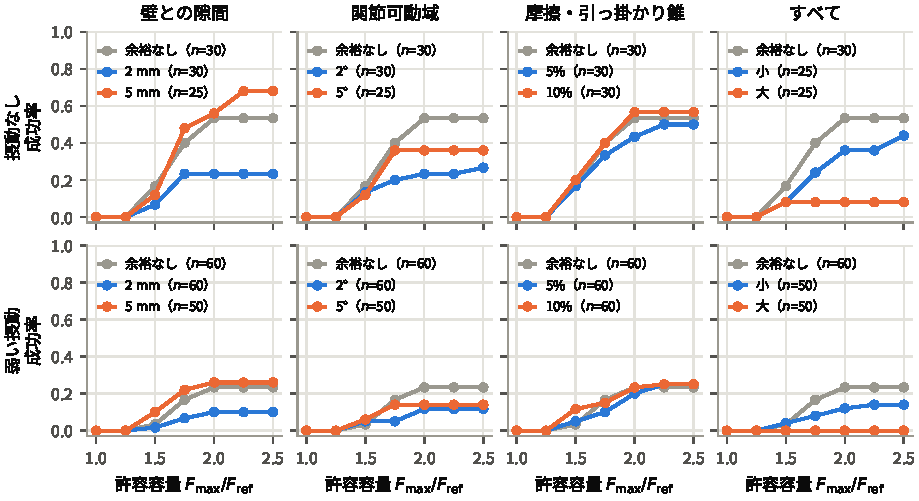
\includegraphics[width=\linewidth]{../results/figs/x3_margins.pdf}
\caption{計画の余裕と再生の成功率（実験 3）．横軸は許容する把持容量，縦軸はその容量での成功率．
上段は状態の摂動なし（離手時刻の誤差 0，$\pm1$，$\pm3$\,ms），下段は弱い摂動（10 通りの乱数）．
二つの捕捉モデルと 3 体格をまとめた．灰色は余裕なしで解き直した計画．}
\label{fig:margins}
\end{figure*}
\begin{table*}[t]
\centering\scriptsize
\caption{計画の余裕（実験 3）．求解成功は収束した計画の数（3 体格 $\times$ 2 捕捉モデル）．
$\Upk$ の増分は余裕なしで解き直した計画に対する値．成功率は $S_{2.0}$ [\%]で，括弧内は試行数．}
\label{tab:margins}
\IfFileExists{tab_x3.tex}{\begin{tabular}{lrrrrr}
\toprule
計画の余裕 & 求解成功 & $\Upk$ の増分 [\%] & 成功率：摂動なし & 弱い摂動 & 強い摂動 \\
\midrule
余裕なし（解き直し） & 6/6 & --- & 53（30） & 23（60） & 2（60） \\
壁 2 mm & 6/6 & -0.4〜+9.8 & 23（30） & 10（60） & 2（60） \\
壁 5 mm & 5/6 & +2.7〜+4.4 & 56（25） & 26（50） & 2（50） \\
関節 2° & 6/6 & -2.1〜+4.8 & 23（30） & 12（60） & 0（60） \\
関節 5° & 5/6 & +0.3〜+4.2 & 36（25） & 14（50） & 0（50） \\
錐 5% & 6/6 & +0.2〜+1.9 & 43（30） & 20（60） & 0（60） \\
錐 10% & 6/6 & -3.0〜+5.4 & 57（30） & 23（60） & 0（60） \\
小さい余裕すべて & 5/6 & +1.8〜+4.8 & 36（25） & 12（50） & 2（50） \\
大きい余裕すべて & 5/6 & +5.6〜+14.5 & 8（25） & 0（50） & 0（50） \\
離手 ±2 ms のシナリオ & 0/6 & --- & --- & --- & --- \\
小さい余裕＋シナリオ & 0/6 & --- & --- & --- & --- \\
大きい余裕＋シナリオ & 0/6 & --- & --- & --- & --- \\
\bottomrule
\end{tabular}
}{（計算中）}
\end{table*}

\subsection{失敗の様相}
図~\ref{fig:failures} に，摂動を加えた再生で見られた失敗の例を示す．
A からの滑落は，体が後ろへ振れて手の反力が錐の外へ出たときに起きる．
壁への接触は，振りの途中で体の一部が A の壁面に 2\,cm を超えて食い込む失敗である．
B の前面への衝突は，飛行の軌道がずれて手が突起の上面ではなく壁の前面に当たる失敗で，
保持中に指が外れる失敗は，捕捉には成功したが，その後の振れ戻りで手の反力が錐の外へ出たものである．
\begin{figure*}[t]
\centering
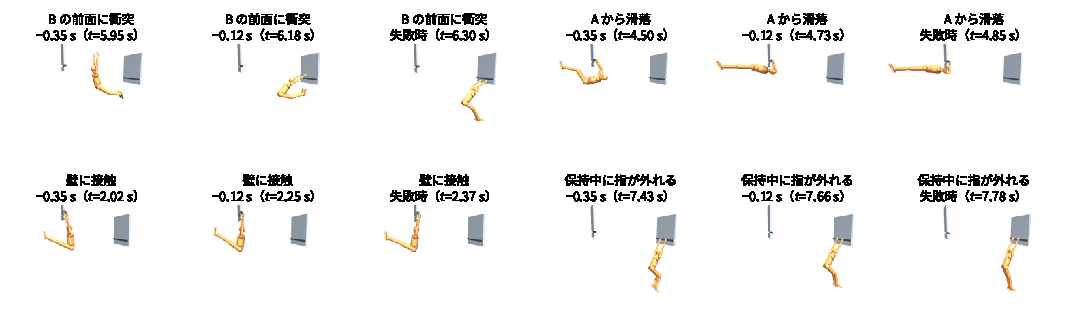
\includegraphics[width=\linewidth]{../results/figs/failures3d.pdf}
\caption{失敗の例（摂動を加えた再生）．各失敗について，失敗の 0.35\,s 前，0.12\,s 前，失敗の瞬間を示す．$t$ は振り開始からの時間．}
\label{fig:failures}
\end{figure*}
